%%%%%%%%%%%%%%%%%%%%%%%%%%%%%%%%%%%%%%%%%%%%%%%
%
% Template per Elaborato di Laurea
% DISI - Dipartimento di Ingegneria e Scienza dell’Informazione
%
% update 2015-09-10
%
% Per la generazione corretta del 
% pdflatex nome_file.tex
% bibtex nome_file.aux
% pdflatex nome_file.tex
% pdflatex nome_file.tex
%
%%%%%%%%%%%%%%%%%%%%%%%%%%%%%%%%%%%%%%%%%%%%%%%

% formato FRONTE RETRO
\documentclass[epsfig,a4paper,11pt,titlepage,twoside,openany]{book}
\usepackage{epsfig}
\usepackage{plain}
\usepackage{setspace}
\usepackage[paperheight=29.7cm,paperwidth=21cm,outer=1.5cm,inner=2.5cm,top=2cm,bottom=2cm]{geometry} % per definizione layout
\usepackage{titlesec} % per formato custom dei titoli dei capitoli

% Pacchetti aggiunti
\usepackage[hyphens]{url}
\usepackage[breaklinks, colorlinks=true, citecolor=red, linkcolor=black, urlcolor=black]{hyperref}
\usepackage{graphicx}
\usepackage[font=small,labelfont=bf]{caption}
\usepackage{subfig}

%%%%%%%%%%%%%%
% supporto lettere accentate
%
%\usepackage[latin1]{inputenc} % per Windows;
\usepackage[utf8x]{inputenc} % per Linux (richiede il pacchetto unicode);
%\usepackage[applemac]{inputenc} % per Mac.

\singlespacing

\usepackage[russian, english]{babel}

\begin{document}

  % nessuna numerazione
  \pagenumbering{gobble} 
  \pagestyle{plain}

\thispagestyle{empty}

\begin{center}
  \begin{figure}[h!]
    \centerline{
\psfig{file=logo_unitn_black_center.eps,width=0.6\textwidth}}
  \end{figure}

  \vspace{2 cm} 

  \LARGE{Dipartimento di Ingegneria e Scienza dell’Informazione\\}

  \vspace{1 cm} 
  \Large{Corso di Laurea in\\
    Informatica
    %Informatica
    %Ingegneria dell'Informazione e delle Comunicazioni
    %Ingegneria dell'Informazione e Organizzazione d'Impresa
    %Ingegneria Elettronica e delle Telecomunicazioni
  }

  \vspace{2 cm} 
  \Large\textsc{Elaborato finale\\} 
  \vspace{1 cm} 
  \Huge\textsc{Soweego\\}
  \Large{\it{solid catalogs and weekee go together}}


  \vspace{2 cm} 
  \begin{tabular*}{\textwidth}{ c @{\extracolsep{\fill}} c }
  \Large{Supervisore} & \Large{Laureando}\\
  \Large{Andrea Passerini}& \Large{Massimo Frasson}\\
  \Large{Marco Fossati}\\
  \end{tabular*}

  \vspace{2 cm} 

  \Large{Anno accademico 2017/2018}
  
\end{center}



  \clearpage
 
%%%%%%%%%%%%%%%%%%%%%%%%%%%%%%%%%%%%%%%%%%%%%%%%%%%%%%%%%%%%%%%%%%%%%%%%%%
%%%%%%%%%%%%%%%%%%%%%%%%%%%%%%%%%%%%%%%%%%%%%%%%%%%%%%%%%%%%%%%%%%%%%%%%%%
%% Nota
%%%%%%%%%%%%%%%%%%%%%%%%%%%%%%%%%%%%%%%%%%%%%%%%%%%%%%%%%%%%%%%%%%%%%%%%%%
%% Sezione Ringraziamenti opzionale
%%%%%%%%%%%%%%%%%%%%%%%%%%%%%%%%%%%%%%%%%%%%%%%%%%%%%%%%%%%%%%%%%%%%%%%%%%
%%%%%%%%%%%%%%%%%%%%%%%%%%%%%%%%%%%%%%%%%%%%%%%%%%%%%%%%%%%%%%%%%%%%%%%%%%
  \clearpage
  \clearpage
  \pagestyle{plain} % nessuna intestazione e pie pagina con numero al centro

  
  % inizio numerazione pagine in numeri arabi
  \mainmatter

%%%%%%%%%%%%%%%%%%%%%%%%%%%%%%%%%%%%%%%%%%%%%%%%%%%%%%%%%%%%%%%%%%%%%%%%%%
%%%%%%%%%%%%%%%%%%%%%%%%%%%%%%%%%%%%%%%%%%%%%%%%%%%%%%%%%%%%%%%%%%%%%%%%%%
%% Nota
%%%%%%%%%%%%%%%%%%%%%%%%%%%%%%%%%%%%%%%%%%%%%%%%%%%%%%%%%%%%%%%%%%%%%%%%%%
%% Si ricorda che il numero massimo di facciate e' 30.
%% Nel conteggio delle facciate sono incluse 
%%   indice
%%   sommario
%%   capitoli
%% Dal conteggio delle facciate sono escluse
%%   frontespizio
%%   ringraziamenti
%%   allegati    
%%%%%%%%%%%%%%%%%%%%%%%%%%%%%%%%%%%%%%%%%%%%%%%%%%%%%%%%%%%%%%%%%%%%%%%%%%
%%%%%%%%%%%%%%%%%%%%%%%%%%%%%%%%%%%%%%%%%%%%%%%%%%%%%%%%%%%%%%%%%%%%%%%%%%

    % indice
    \tableofcontents
    \clearpage
    
    
          
    % gruppo per definizone di successione capitoli senza interruzione di pagina
    \begingroup
      % nessuna interruzione di pagina tra capitoli
      % ridefinizione dei comandi di clear page
      \renewcommand{\cleardoublepage}{} 
      \renewcommand{\clearpage}{} 
      % redefinizione del formato del titolo del capitolo
      % da formato
      %   Capitolo X
      %   Titolo capitolo
      % a formato
      %   X   Titolo capitolo
      
      \titleformat{\chapter}
        {\normalfont\Huge\bfseries}{\thechapter}{1em}{}
        
      \titlespacing*{\chapter}{0pt}{0.59in}{0.02in}
      \titlespacing*{\section}{0pt}{0.20in}{0.02in}
      \titlespacing*{\subsection}{0pt}{0.10in}{0.02in}
      
      % sommario
      \clearpage
\newpage
\mbox{~}
\clearpage
\newpage

\chapter*{Summary} % senza numerazione
\label{abstract}
Wikipedia and \textbf{Wikidata} are open source collaborative projects with the goal of collecting and sharing general knowledge. While the former is intended for humans, the latter caters for \textbf{machine-readable data}. Both are not meant to contain \textit{original research}.\footnote{\url{https://en.wikipedia.org/wiki/Wikipedia:No_original_research}}\footnote{\url{https://www.wikidata.org/wiki/Wikidata:What_Wikidata_is_not}} Original research means that no reliable or published material exists referring to reported facts, allegations or ideas.
Such design decision entails that Wikipedia and Wikidata content should be supported by references to external sources.
Nevertheless, \texttt{Wikidata} suffers from a \textbf{lack of references}.
The \textbf{soweego} project aims at mitigating the issue by \textbf{linking} \texttt{Wikidata} to a set of trustworthy target \textbf{catalogs}, a task that can be cast as a record linkage problem.
As a result, \textbf{references and new content} may be mined from these catalogs after the linking.

\textbf{Record linkage}\footnote{\url{https://en.wikipedia.org/wiki/Record_linkage\#Probabilistic_record_linkage}} must cope with several challenges: inaccurate data, heterogeneous data precision, and ambiguity, just to name the key ones.
% Homonyms are the very first issue to deal with, as much as people's second names notation (extended, short, missing).
These challenges can be addressed by comparing other data attributes, such as dates and locations. However, there is no guarantee that \texttt{Wikidata} and the target will share any attribute. \texttt{soweego} addresses the issue by working on a common set of attributes, but for the sake of generalization it supports target-specific ones.

This thesis details a set of deterministic techniques for record linkage: \textit{perfect full name match}; \textit{perfect name with birth and death dates match}; \textit{perfect cross-catalog link match}; \textit{tokenized cross catalog link match}; \textit{normalized full names match}.
Specifically, we designed them to work on the common set of attributes, and we evaluate the results obtained picking the \texttt{MusicBrainz} as target database.
We observe that \textit{URLs to external sources} and \textit{dates} attributes provide a relatively high precision.
Hence, the output produced by these techniques has been added to \texttt{Wikidata}.

Our work on the aforementioned techniques represents the fundamental building blocks and knowledge to scale up from deterministic algorithms to probabilistic ones.
We summarize our contributions to the \texttt{soweego} project as follows.
\begin{itemize}
    \item Analysis of the long tail of candidate target catalogs;
    \item development of the facility to import the \texttt{MusicBrainz} dump in the system;
    \item implementation of the baseline techniques for \texttt{MusicBrainz};
    \item performance evaluation;
    \item software packaging in a portable environment;
    \item intervention to all technical discussions.
\end{itemize}

\pagebreak


%%%%%%%%%%%%%%%%%%%%%%%%%%%%%%%%%%%%%%%%%%%%%%%%%%%%%%%%%%%%%%%%%%%%%%%%%%
%%%%%%%%%%%%%%%%%%%%%%%%%%%%%%%%%%%%%%%%%%%%%%%%%%%%%%%%%%%%%%%%%%%%%%%%%%
%% Nota
%%%%%%%%%%%%%%%%%%%%%%%%%%%%%%%%%%%%%%%%%%%%%%%%%%%%%%%%%%%%%%%%%%%%%%%%%%
%% Sommario e' un breve riassunto del lavoro svolto dove si descrive 
%% l’obiettivo, l’oggetto della tesi, le metodologie e 
%% le tecniche usate, i dati elaborati e la spiegazione delle conclusioni 
%% alle quali siete arrivati.
%% Il sommario dell’elaborato consiste al massimo di 3 pagine e deve contenere le seguenti informazioni: 
%%   contesto e motivazioni
%%   breve riassunto del problema affrontato
%%   tecniche utilizzate e/o sviluppate
%%   risultati raggiunti, sottolineando il contributo personale del laureando/a
%%%%%%%%%%%%%%%%%%%%%%%%%%%%%%%%%%%%%%%%%%%%%%%%%%%%%%%%%%%%%%%%%%%%%%%%%%
%%%%%%%%%%%%%%%%%%%%%%%%%%%%%%%%%%%%%%%%%%%%%%%%%%%%%%%%%%%%%%%%%%%%%%%%%%      
      
      %%%%%%%%%%%%%%%%%%%%%%%%%%%%%%%%
      % lista dei capitoli
      %
      % \input oppure \include
      %
      \clearpage
\newpage
\mbox{~}
\clearpage
\newpage

\chapter{Introduction}
\label{cha:intro}
In 2018, the English Wikipedia has been visited 207.83 billions of times, a 4.73\% increase year by year.\footnote{\url{https://stats.wikimedia.org/v2/\#/en.wikipedia.org/reading/total-page-views/normal|bar|1-Year|~total}} This shows that Wikipedia is one of the key tools for enhancing people knowledge, due to the easily accessible free information. However, the unstructured nature of its content does not enable straightforward machine processing.
% For this reason, projects like Wikidata were created.
Wikidata\footnote{\url{https://www.wikidata.org/}} acts as central storage for structured data of its Wikimedia sister projects, including Wikipedia, Wikivoyage, Wikisource, and others.

Data quality is a crucial factor for the trustworthiness of Wikipedia and Wikidata content. In fact, Wikipedia provides mature citation guidelines to enforce high quality standard.\footnote{\url{https://en.wikipedia.org/wiki/Wikipedia:Citing_sources}}
Likewise, Wikidata allows to store references to (ideally authoritative) sources along with its data.

Nevertheless, \textbf{less than a quarter} of the Wikidata knowledge base (KB) statements currently has a reference to \textbf{non-wiki} sources, and roughly an \textbf{half} of them is totally \textbf{unreferenced}.\footnote{\url{https://docs.google.com/presentation/d/1XX-yzT98fglAfFkHoixOI1XC1uwrS6f0u1xjdZT9TYI/edit?usp=sharing}, slides 15 to 19}
The problem can be alleviated in several ways: we could encourage the community to focus on the referencing task. Another option could be the alignemnt of Wikidata entities to a set of external databases, which can be automated by software. This is a particularly interesting option because it provides a repeatable process.

\begin{figure}[t]
  \begin{center}
   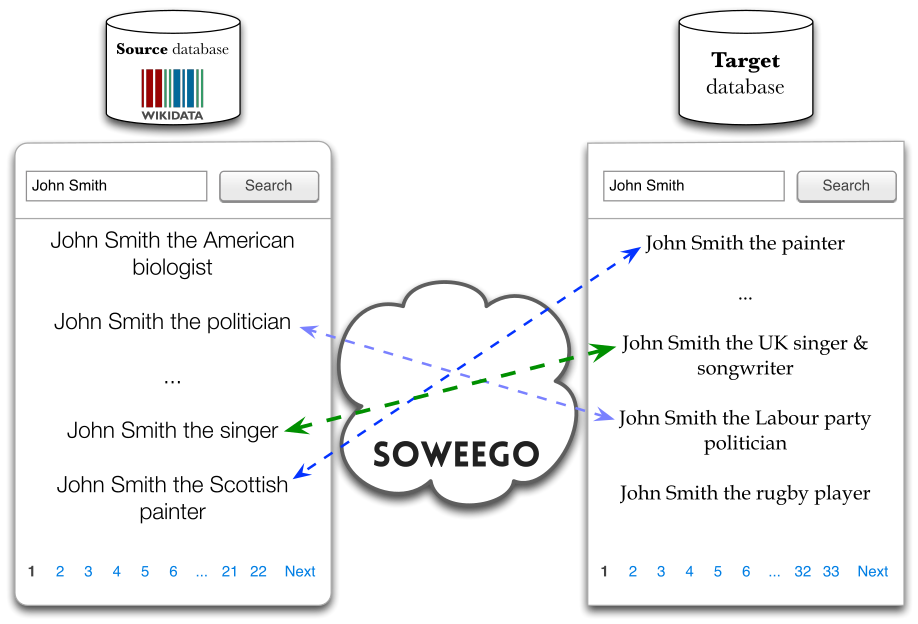
\includegraphics[height=200px]{images/matchexample.png}
   \captionof{figure}{\texttt{soweego} creates a connection (read performs disambiguation) between entries of the source database (Wikidata) and a target database. Image by \href{https://meta.wikimedia.org/wiki/User:Hjfocs}{\texttt{Hjfocs}}, \href{https://creativecommons.org/licenses/by-sa/4.0/deed.en}{CC BY-SA 4.0}}
   \label{fig:soweegomatch}
  \end{center}
\end{figure}

We define the problem as follows: given a Wikidata entity, find a suitable match in the target database.
This is not a trivial task, with homonyms being the first challenge.
For instance, suppose we would like to know more about the singer \textit{John Smith}.
We type the name into the Wikidata search box: multiple results appear, and it takes a while to find the person we are looking for.
Unfortunately, Wikidata does not hold much information about him and our search moves to another database, like MusicBrainz\footnote{\url{https://musicbrainz.org}}.
We must repeat the same procedure as with Wikidata, and after some digging, we manage to find John Smith the singer. This is a match: the MusicBrainz entity can be linked to Wikidata.
\texttt{soweego} aims at solving the issue at a large scale, via disambiguation of a source Wikidata entity to a target database entry. Figure~\ref{fig:soweegomatch} depicts the solution.

Wikidata entities are designed to store this kind of links. In particular, entities like John Smith are called \textit{items} and each of them is composed of an \textit{identifier}, a \textit{fingerprint}, and a set of \textit{statements}.\footnote{\url{https://www.mediawiki.org/wiki/Wikibase/DataModel/Primer}}
Each statement is broken down into \textit{claims} (i.e., property, value pairs) and optional \textit{references} (i.e., the sources of the factual information).
For instance, John Smith could have the claim (\texttt{given name}, \texttt{John}), together with its reference (\texttt{stated in}, \texttt{Duckburg Municipality archive}).
The identifier links to external sources are expressed as claims too.
The John Smith match between Wikidata and MusicBrainz would be e.g., expressed as a claim over the Wikidata item with identifier \texttt{Q666} (\texttt{MusicBrainz artist ID}, \texttt{77a1c579-3532-491c-86bd-595ddd4780cc}), where the latter value corresponds to the MusicBrainz identifier.

Officially, \texttt{soweego} has the following goals:\footnote{\url{https://meta.wikimedia.org/wiki/Grants:Project/Hjfocs/soweego\#Project_goals}}
\begin{enumerate}
    \item to ensure live maintenance of identifiers for people in Wikidata, via link validation;
    \item to develop a set of linking techniques that align people in Wikidata to corresponding identifiers in external catalogs;
    \item to ingest links into Wikidata, either through a bot (confident links), or mediated by curation (non-confident links);
    \item to achieve exhaustive coverage (ideally 100\%) of identifiers over 4 large-scale trusted catalogs;
    \item to deliver a self-sustainable application that can be easily operated by the community after the end of the project.
\end{enumerate}

The remainder of this thesis is structured as follows. In section \ref{cha:2} we report a brief review of the state of the art. The preliminary analysis of the candidate targets is detailed in section \ref{cha:3}. Section \ref{cha:4} describes the project architecture with a focus on the matching strategies, which we evaluate against MusicBrainz in section \ref{cha:5}. We draw our conclusions in section \ref{cha:conclusioni}.


      \chapter{Related work}
\label{cha:2}
The alignment of Wikidata to structured authoritative databases can yield a lot of references, even if it is a demanding task. In fact, the labels can be the same among Wikidata and the chosen database, but there could be homonyms. To overcome the issue we need to exploit other attributes in addition to labels. Choosing these extra attributes is an issue itself since Wikidata and the target database have probably different attribute sets. It is not even assumable that the attributes will be the same among all the entities in the same KB, like Wikidata. 

\texttt{SocialLink}, a system that aligns knowledge base entries of people and organizations to the  corresponding social media profiles\cite{DBLP:conf/semweb/NechaevCG17a}, shares the same challenges. \texttt{SocialLink} addressed them by picking a minimal subset of attributes: name, difference between person and organization and temporal information that tells if the entity is alive/existent. Similarly, we chose full name, birth and death dates, and a set of URLs related to the entity. Though, we let the chance of adding target specific attributes, unlike \texttt{SocialLink}.

The exceeding attributes can improve the linking process, but they can also be exploited in a KB population task. In fact, mapping the semantics of these attributes against the Wikidata ontology would result in the addition of referenced statements. These statements cannot replace the work done by \texttt{StrepHit}\cite{DBLP:journals/semweb/FossatiDG18} or the one described in \cite{self:SocialLink/TypePrediction}, but is still a contribution. Unlike us, they work on unstructured data, such as full text or social media content.

An existing \texttt{SocialLink} improvement \cite{self:SocialLink/Embeddings} exploits an enhanced representation of the social graph, compared to \cite{DBLP:conf/sac/NechaevCG17}. Despite the improvement, \cite{self:SocialLink/Embeddings} will not be helpful in soweego, since we cannot assume the availability of any social graph data.

The alignment task deals with a lot of queries on those attributes, so working with the targets APIs could be an issue: APIs usage is restricted and also web requests bring latency in code execution. Like SocialLink\cite{DBLP:conf/sac/NechaevCG17}, we work with a custom indexed database, but we have been able to populate it through the target dumps.


      \chapter{Preliminary analysis}
\label{cha:3}
The very first task of this project is to select the target databases.\footnote{\url{https://meta.wikimedia.org/wiki/Grants:Project/Hjfocs/soweego\#Work_package}} We see two directions here: either we focus on a few big and well known targets as per the project proposal, or we can try to find a technique to link a lot of small ones from the long tail, as suggested by \texttt{ChristianKl}\footnote{\url{https://meta.wikimedia.org/wiki/Grants_talk:Project/Hjfocs/soweego\#Target_databases_scalability}}.

We used \textbf{SQID}\footnote{\url{https://tools.wmflabs.org/sqid/\#/browse?type=properties}} as a starting point to get a list of people databases that are already used in Wikidata, sorted in descending order of usage.\footnote{\textit{Select datatype} set to \textit{ExternalId}, \textit{Used for class} set to \textit{human Q5}} This is useful to split the candidates into \textit{big} and \textit{small} fishes, namely the head and the (long) tail of the result list respectively.

Quoting \texttt{ChristianKl}, it would be ideal to create a configurable tool that enables users to add links to \textit{new databases in a reasonable time-frame} (standing for no code writing). Consequently, we carried out the following investigation: we considered as small fishes all the entries in \textbf{SQID} with an external ID data type, used for class  human (Q5)\footnote{\url{https://www.wikidata.org/wiki/Q5}}, and with \textbf{less than 15 uses in statements}. It results that some critical issues need to be solved to follow this direction, as described in the following lines.

The analysis of a small fish can be broken down into a set of steps. This is also useful to translate the process into software and to make each step flexible enough for dealing with the heterogeneity of the long tail targets. The steps have been implemented into a piece of software by \texttt{MaxFrax96}.\footnote{\url{https://github.com/MaxFrax/Evaluation}}

\section{Retrieving the dump}
\label{cha:31}
The naive technique to link two database is, for each entity in the first one, doing a look up into the second one. Since databases contain a lot of data, we need the dumps to avoid APIs restrictions and slow computation due to connection latency.
Moreover we focus on people, it is therefore necessary to obtain the appropriate dump for each small fish we consider.

\subsection{Problem}
\label{cha:311}
In the real world, such a trivial step raises a first critical issue: not all the database websites give us the chance to download the dump.

\subsection{Solutions}
\label{cha:312}
A non technical complexity solution would be contacting the databases administrators and discuss dump releases for Wikidata, however requires a lot of manual work becoming hard to scale up.

On the contrary, building autonomously the dump would scale up much better. Given a valid URI for each entity, we can re-create the dump. However, this is not trivial to generalize: sometimes it is impossible to retrieve the list of entities, sometimes the URIs are merely HTML pages that require Web scraping. For instance \texttt{Welsh Rugby Union men's player ID (P3826)}\footnote{\url{https://www.wikidata.org/wiki/Property:P3826}}, \texttt{Berlinische Galerie artist ID (P4580)}\footnote{\url{https://www.wikidata.org/wiki/Property:P4580}}, \texttt{FAI ID (P4556)}\footnote{\url{https://www.wikidata.org/wiki/Property:P4556}}, at the time of writing, need scraping for both the list of entities and each entity; \texttt{Debrett's People of Today ID (P2255)}\footnote{\url{https://www.wikidata.org/wiki/Property:P2255}}, \texttt{AGORHA event identifier (P2345)}\footnote{\url{https://www.wikidata.org/wiki/Property:P2345}}, at time of writing, do not seem to expose any list of people.

\section{Mapping to Wikidata}
\label{cha:32}
The long tail is roughly broken down as follows:
\begin{itemize}
    \item XML;
    \item JSON;
    \item RDF;
    \item HTML pages with styling and whatever a Web page can contain.
\end{itemize}

\subsection{Problem}
\label{cha:321}
Formats are heterogeneous. We focus on open data and RDF, as dealing with custom APIs is out of scope for this investigation. We also hope that the open data trend of recent years would help us. However, a manual scan of the small fishes yielded poor results. There were 56 targets in our long tail, out of \textbf{16} randomly picked candidates, only \texttt{YCBA agent ID}\footnote{\url{https://www.wikidata.org/wiki/Property:P4169}} was in RDF, and has thousands of uses in statements at the time of writing this report.
\subsection{Solution}
\label{cha:322}
To define a way (by scripting for instance) to translate each input format into a standard project-wide one. This could be achieved during the next step, namely ontology mapping between a given small fish and Wikidata.

\section{Handling the format}
\label{cha:33}
Linking Wikidata items to target entities requires a mapping between both meta-data/schemas.

\subsection{Solution}
\label{cha:331}
The mapping can be manually defined by the community: a piece of software will then apply it. To implement this step, we also need the common data format described above.

\subsection{Side note: available entity meta-data}
\label{cha:332}
Small fishes may contain entity meta-data which are likely to be useful for automatic matching. The entity linking process may dramatically improve if the system is able to mine extra property mappings. This is obvious when meta-data are in different languages, but in general we cannot be sure that two different databases hold the same set of properties, if they have some in common.

\section{Conclusion}
\label{cha:34}
It is out of scope for the project to perform entity linking over the whole set of small fishes. On the other hand, it may make sense to build a system that lets the community plug in new small fishes with relative ease. Nevertheless, this would require a reshape of the original proposal, which comes with its own risks:
\begin{itemize}
\item it is probably not a safe investment of resources;
\item eventual results would not be in the short term, as they would require a lot of work to create a flexible system for everybody's needs;
\item it is likely that the team is not facing eventual extra problems in this phase.
\end{itemize}

Most importantly, a system to plug new small fishes \textbf{already exists}. \textbf{Mix'n'match}\footnote{\url{https://tools.wmflabs.org/mix-n-match/}} is specifically designed for the task.\footnote{\url{http://magnusmanske.de/wordpress/?p=471}}. Instead of reinventing the wheel, we joined efforts with our advisor \texttt{Magnus Manske}\footnote{\url{https://meta.wikimedia.org/wiki/User:Magnus_Manske}} in his work on big fishes\footnote{\url{http://magnusmanske.de/wordpress/?p=478}}


      \chapter{System architecture}
\label{cha:4}

Soweego is a pipeline that accomplishes several tasks in order to link entities between Wikidata and the target database. For the purpose of the following description, the target database will be MusicBrainz.\footnote{\url{https://musicbrainz.org}} MusicBrainz is a community-maintained open source encyclopedia of music information.\footnote{\url{https://musicbrainz.org/doc/About}} In particular, the relevant data for the pipeline are the artists, since they're humans.
\todo{Va esteso?}

\section{Importer}
\label{cha:41}
The importer is the pipeline's module in charge of downloading the latest target database dump and store it in a database. The import phase does not work on the data as is, but treats it to extract only the desired slice. Since soweego aims to work against different databases, there's a configurable middleware that handles the translation from the desired database to the project's format. The format consists in a set of basic attributes:
\begin{itemize}
    \item \textit{Catalog ID}, the identifier of the entity in the target database
    \item \textit{Label}, the full name
    \item \textit{Birth Date}
    \item \textit{Birth date precision}
    \item \textit{Death Date}
    \item \textit{Death date precision}
\end{itemize}
The schema is extendable for each source database, however the set of shared attributes enables having procedures in common among all the sources.

A common issue, in music databases above all, is people having   multiple names, known as \textbf{aliases}. The schema easily handles them by treating the aliases as standalone people. Clearly these standalone records will share all the original name's data, except the label.

BaseLink -> magari piccolo ER

Mapping di Musicbrainz


\section{Linker}
\label{cha:42}

Al momento sistema rule based per creare una baseline

Perfect name

birth and death dates

Damerau-Levenshtein

Levenshtein

Jaro-Winkler

Cross catalog link (including sitelinks)

Extension Token similarity for urls



\section{Ingestor}
\label{cha:43}

\section{Validator}
\label{cha:44}

\begin{figure}
  \begin{center}
   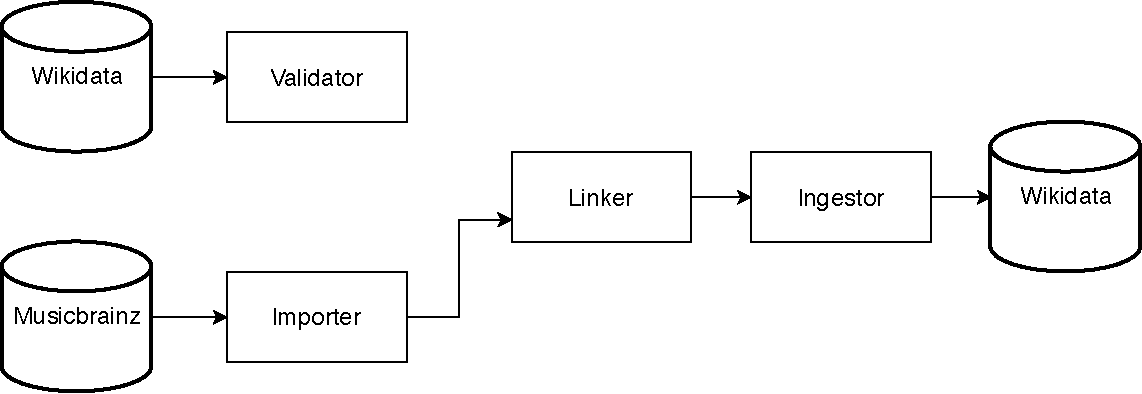
\includegraphics[width=\textwidth]{images/architecture.pdf}
   \captionof{figure}{Soweego architecture overview}
  \end{center}
\end{figure}


      \chapter{Results}
\label{cha:789}
Lorem ipsum dolor sit amet, consectetur adipiscing elit. Donec sed nunc orci. Aliquam nec nisl vitae sapien pulvinar dictum quis non urna. Suspendisse at dui a erat aliquam vestibulum. Quisque ultrices pellentesque pellentesque. Pellentesque egestas quam sed blandit tempus. Sed congue nec risus posuere euismod. Maecenas ut lacus id mauris sagittis egestas a eu dui. Class aptent taciti sociosqu ad litora torquent per conubia nostra, per inceptos himenaeos. Pellentesque at ultrices tellus. Ut eu purus eget sem iaculis ultricies sed non lorem. Curabitur gravida dui eget ex vestibulum venenatis. Phasellus gravida tellus velit, non eleifend justo lobortis eget. 


\section{Cras in aliquam quam, et}
\label{sec:456}
Lorem ipsum dolor sit amet, consectetur adipiscing elit. Donec sed nunc orci. Aliquam nec nisl vitae sapien pulvinar dictum quis non urna. Suspendisse at dui a erat aliquam vestibulum. Quisque ultrices pellentesque pellentesque. Pellentesque egestas quam sed blandit tempus. Sed congue nec risus posuere euismod. Maecenas ut lacus id mauris sagittis egestas a eu dui. Class aptent taciti sociosqu ad litora torquent per conubia nostra, per inceptos himenaeos. Pellentesque at ultrices tellus. Ut eu purus eget sem iaculis ultricies sed non lorem. Curabitur gravida dui eget ex vestibulum venenatis. Phasellus gravida tellus velit, non eleifend justo lobortis eget.


\subsection{Sed pulvinar placerat enim, a}
\label{sec:00456}
Lorem ipsum dolor sit amet, consectetur adipiscing elit. Donec sed nunc orci. Aliquam nec nisl vitae sapien pulvinar dictum quis non urna. Suspendisse at dui a erat aliquam vestibulum. Quisque ultrices pellentesque pellentesque. Pellentesque egestas quam sed blandit tempus. Sed congue nec risus posuere euismod. Maecenas ut lacus id mauris sagittis egestas a eu dui. Class aptent taciti sociosqu ad litora torquent per conubia nostra, per inceptos himenaeos. Pellentesque at ultrices tellus. Ut eu purus eget sem iaculis ultricies sed non lorem. Curabitur gravida dui eget ex vestibulum venenatis. Phasellus gravida tellus velit, non eleifend justo lobortis eget.


\section{Vivamus hendrerit imperdiet ex. Vivamus}
\label{sec:123}
Lorem ipsum dolor sit amet, consectetur adipiscing elit. Donec sed nunc orci. Aliquam nec nisl vitae sapien pulvinar dictum quis non urna. Suspendisse at dui a erat aliquam vestibulum. Quisque ultrices pellentesque pellentesque. Pellentesque egestas quam sed blandit tempus. Sed congue nec risus posuere euismod. Maecenas ut lacus id mauris sagittis egestas a eu dui. Class aptent taciti sociosqu ad litora torquent per conubia nostra, per inceptos himenaeos. Pellentesque at ultrices tellus. Ut eu purus eget sem iaculis ultricies sed non lorem. Curabitur gravida dui eget ex vestibulum venenatis. Phasellus gravida tellus velit, non eleifend justo lobortis eget.



      \chapter{Conclusion}
\label{cha:conclusioni}
\texttt{Wikidata} is a general-purpose structured knowledge base housed by the Wikimedia Foundation.\footnote{\url{https://wikimediafoundation.org/}}
Its community is becoming more and more active in data curation: in the last year, the number of edits increased by 75.26\%, compared to the previous year.\footnote{\url{https://stats.wikimedia.org/v2/\#/wikidata.org/contributing/edits/normal|bar|1-Year|~total}} Despite such increased effort, Wikidata still suffers from a lack of references that support the trustworthiness of its content: currently, only less than \textbf{a quarter} of it has a reference to \textbf{non-wiki} sources and roughly a \textbf{half} is totally \textbf{unreferenced}.\footnote{\url{https://docs.google.com/presentation/d/1XX-yzT98fglAfFkHoixOI1XC1uwrS6f0u1xjdZT9TYI/edit?usp=sharing}, slides 15 to 19}

In this thesis, we described the first development iteration of \texttt{soweego}, an automatic linking system for large catalogs that aims at filling the reference gap.
Specifically, we illustrated the  \texttt{Wikidata} - \texttt{MusicBrainz} use case.
Our contribution boils down to a set of core building blocks, the most prominent being the \textit{linker}, plus the \textit{ingestor}, \textit{validator}, and \textit{importer} components, which lay the foundation for the final product.
Despite the project is only 3 months old, with a planned duration of 1 year, we managed to add \textbf{several hundreds of high-quality matches}\footnote{\url{https://www.wikidata.org/wiki/Special:Contributions/Soweego_bot}} to \texttt{Wikidata}.

In the \textit{linker} module, we explored rule-based matching strategies, which serve as a baseline system for construction and comparison  of future machine learning-based strategies.
Furthermore, we acquired insights on the actual data quality of \texttt{Wikidata} and earned expertise on the key features for improvement of the linking process.
As described in Section \ref{cha:5}, links are a very precise feature to rely upon. Although dates perform well, they are not a valid standalone feature: on the other hand, they have a positive impact on the precision if they are combined to other ones.
Finally, full name matching is a risky feature, as expected, creating a lot of false positives.

The very next steps will focus on the improvement of existing strategies.
First, the \textit{cross-database URL} strategy introduced in Section \ref{cha:423} will consume \textit{official homepages} of \texttt{Wikidata} entities, as well as the \textit{ISNI code} of the \texttt{MusicBrainz} ones. Moreover, we will investigate how tokenization in \textit{normalized names} strategy (cf. Section \ref{cha:424}) can be better exploited.

Future work will include deeper research in the record linkage literature to improve the system, with a special attention on probabilistic approaches.
Machine learning could be an interesting direction to take, as shown in \cite{DBLP:conf/semweb/NechaevCG17a}.
The immediate goal is to obtain a confidence score for each computed match, expressed as probability.
The baseline strategies could become our features in a machine learning-based solution.
Moreover, inspired by \cite{DBLP:conf/semweb/NechaevCG17a}, we plan to use the full names strategies to select a subset of entities as input for the linking phase.
In this way, our system would perform faster, thanks to the lower number of entities to check. This is possible just because we verified that full names matches tend to be a super set of the other strategies matches.

\clearpage
\newpage
\mbox{~}
\clearpage
\newpage
      %\input{capitolo4}
      
      
    \endgroup


    % bibliografia in formato bibtex
    %
    % aggiunta del capitolo nell'indice
    \addcontentsline{toc}{chapter}{Bibliografia}
    % stile con ordinamento alfabetico in funzione degli autori
    \bibliographystyle{plain}
    \bibliography{biblio}
%%%%%%%%%%%%%%%%%%%%%%%%%%%%%%%%%%%%%%%%%%%%%%%%%%%%%%%%%%%%%%%%%%%%%%%%%%
%%%%%%%%%%%%%%%%%%%%%%%%%%%%%%%%%%%%%%%%%%%%%%%%%%%%%%%%%%%%%%%%%%%%%%%%%%
%% Nota
%%%%%%%%%%%%%%%%%%%%%%%%%%%%%%%%%%%%%%%%%%%%%%%%%%%%%%%%%%%%%%%%%%%%%%%%%%
%% Nella bibliografia devono essere riportati tutte le fonti consultate 
%% per lo svolgimento della tesi. La bibliografia deve essere redatta 
%% in ordine alfabetico sul cognome del primo autore. 
%% 
%% La forma della citazione bibliografica va inserita secondo la fonte utilizzata:
%% 
%% LIBRI
%% Cognome e iniziale del nome autore/autori, la data di edizione, titolo, casa editrice, eventuale numero dell’edizione. 
%% 
%% ARTICOLI DI RIVISTA
%% Cognome e iniziale del nome autore/autori, titolo articolo, titolo rivista, volume, numero, numero di pagine.
%% 
%% ARTICOLI DI CONFERENZA
%% Cognome e iniziale del nome autore/autori (anno), titolo articolo, titolo conferenza, luogo della conferenza (città e paese), date della conferenza, numero di pagine. 
%% 
%% SITOGRAFIA
%% La sitografia contiene un elenco di indirizzi Web consultati e disposti in ordine alfabetico. 
%% E’ necessario:
%%   Copiare la URL (l’indirizzo web) specifica della pagina consultata
%%   Se disponibile, indicare il cognome e nome dell’autore, il titolo ed eventuale sottotitolo del testo
%%   Se disponibile, inserire la data di ultima consultazione della risorsa (gg/mm/aaaa).    
%%%%%%%%%%%%%%%%%%%%%%%%%%%%%%%%%%%%%%%%%%%%%%%%%%%%%%%%%%%%%%%%%%%%%%%%%%
%%%%%%%%%%%%%%%%%%%%%%%%%%%%%%%%%%%%%%%%%%%%%%%%%%%%%%%%%%%%%%%%%%%%%%%%%%
    

    %\titleformat{\chapter}
    %    {\normalfont\Huge\bfseries}{Allegato \thechapter}{1em}{}
    % sezione Allegati - opzionale
    %\appendix
    %\chapter{Titolo primo allegato}

Lorem ipsum dolor sit amet, consectetur adipiscing elit. Donec sed nunc orci. Aliquam nec nisl vitae sapien pulvinar dictum quis non urna. Suspendisse at dui a erat aliquam vestibulum. Quisque ultrices pellentesque pellentesque. Pellentesque egestas quam sed blandit tempus. Sed congue nec risus posuere euismod. Maecenas ut lacus id mauris sagittis egestas a eu dui. Class aptent taciti sociosqu ad litora torquent per conubia nostra, per inceptos himenaeos. Pellentesque at ultrices tellus. Ut eu purus eget sem iaculis ultricies sed non lorem. Curabitur gravida dui eget ex vestibulum venenatis. Phasellus gravida tellus velit, non eleifend justo lobortis eget. 

\section{Titolo}
Lorem ipsum dolor sit amet, consectetur adipiscing elit. Donec sed nunc orci. Aliquam nec nisl vitae sapien pulvinar dictum quis non urna. Suspendisse at dui a erat aliquam vestibulum. Quisque ultrices pellentesque pellentesque. Pellentesque egestas quam sed blandit tempus. Sed congue nec risus posuere euismod. Maecenas ut lacus id mauris sagittis egestas a eu dui. Class aptent taciti sociosqu ad litora torquent per conubia nostra, per inceptos himenaeos. Pellentesque at ultrices tellus. Ut eu purus eget sem iaculis ultricies sed non lorem. Curabitur gravida dui eget ex vestibulum venenatis. Phasellus gravida tellus velit, non eleifend justo lobortis eget. 

\subsection{Sottotitolo}
Lorem ipsum dolor sit amet, consectetur adipiscing elit. Donec sed nunc orci. Aliquam nec nisl vitae sapien pulvinar dictum quis non urna. Suspendisse at dui a erat aliquam vestibulum. Quisque ultrices pellentesque pellentesque. Pellentesque egestas quam sed blandit tempus. Sed congue nec risus posuere euismod. Maecenas ut lacus id mauris sagittis egestas a eu dui. Class aptent taciti sociosqu ad litora torquent per conubia nostra, per inceptos himenaeos. Pellentesque at ultrices tellus. Ut eu purus eget sem iaculis ultricies sed non lorem. Curabitur gravida dui eget ex vestibulum venenatis. Phasellus gravida tellus velit, non eleifend justo lobortis eget. 


\chapter{Titolo secondo allegato}

Lorem ipsum dolor sit amet, consectetur adipiscing elit. Donec sed nunc orci. Aliquam nec nisl vitae sapien pulvinar dictum quis non urna. Suspendisse at dui a erat aliquam vestibulum. Quisque ultrices pellentesque pellentesque. Pellentesque egestas quam sed blandit tempus. Sed congue nec risus posuere euismod. Maecenas ut lacus id mauris sagittis egestas a eu dui. Class aptent taciti sociosqu ad litora torquent per conubia nostra, per inceptos himenaeos. Pellentesque at ultrices tellus. Ut eu purus eget sem iaculis ultricies sed non lorem. Curabitur gravida dui eget ex vestibulum venenatis. Phasellus gravida tellus velit, non eleifend justo lobortis eget. 

\section{Titolo}
Lorem ipsum dolor sit amet, consectetur adipiscing elit. Donec sed nunc orci. Aliquam nec nisl vitae sapien pulvinar dictum quis non urna. Suspendisse at dui a erat aliquam vestibulum. Quisque ultrices pellentesque pellentesque. Pellentesque egestas quam sed blandit tempus. Sed congue nec risus posuere euismod. Maecenas ut lacus id mauris sagittis egestas a eu dui. Class aptent taciti sociosqu ad litora torquent per conubia nostra, per inceptos himenaeos. Pellentesque at ultrices tellus. Ut eu purus eget sem iaculis ultricies sed non lorem. Curabitur gravida dui eget ex vestibulum venenatis. Phasellus gravida tellus velit, non eleifend justo lobortis eget. 

\subsection{Sottotitolo}
Lorem ipsum dolor sit amet, consectetur adipiscing elit. Donec sed nunc orci. Aliquam nec nisl vitae sapien pulvinar dictum quis non urna. Suspendisse at dui a erat aliquam vestibulum. Quisque ultrices pellentesque pellentesque. Pellentesque egestas quam sed blandit tempus. Sed congue nec risus posuere euismod. Maecenas ut lacus id mauris sagittis egestas a eu dui. Class aptent taciti sociosqu ad litora torquent per conubia nostra, per inceptos himenaeos. Pellentesque at ultrices tellus. Ut eu purus eget sem iaculis ultricies sed non lorem. Curabitur gravida dui eget ex vestibulum venenatis. Phasellus gravida tellus velit, non eleifend justo lobortis eget. 




\end{document}
